%!TEX TS-program = pdflatexmk

% Copyright (c) 2018 - 2022, Martin Scheidt (ISC license)
% Permission to use, copy, modify, and/or distribute this file for any purpose with or without fee is hereby granted, provided that the above copyright notice and this permission notice appear in all copies.

\documentclass[tikz,border=2]{standalone}
\usepackage{tikz-trackschematic} % loading the library

\begin{document}
  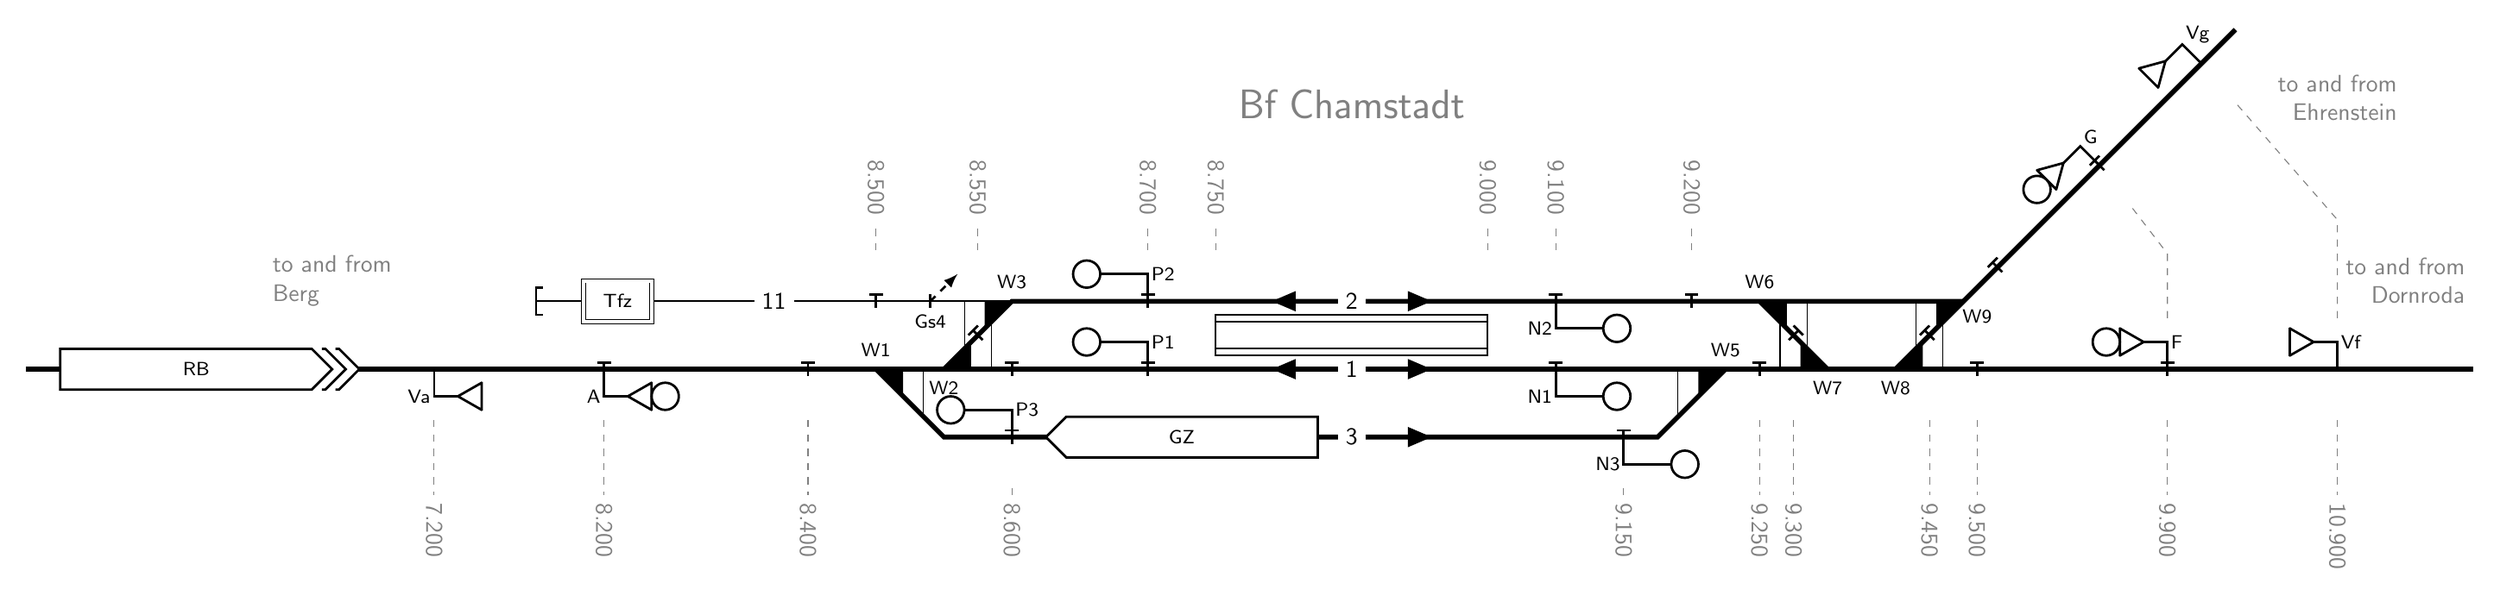
\begin{tikzpicture}[font=\sffamily]
  { % station names
    \tikzset{every node/.style={foreground!50!background}};
    \node[right,align=left] at ( 5,1.3) {to and from\\ Berg};
    \node                   at (21,3.9) {{\LARGE Bf Chamstadt}};
    \node[left,align=right] at (37.5,1.3) {to and from\\ Dornroda};
    \node[left,align=right] at (36.5,4.0) {to and from\\ Ehrenstein};
  }
  % coordinates
  \coordinate (A)  at ( 1.5, 0);
  \coordinate (B)  at (37.5, 0);
  \coordinate (C)  at (34  , 5);

  \coordinate (E1) at ( 9  , 1);

  \coordinate (Y1) at (14  , 0);
  \coordinate (Y2) at (15  , 0);
  \coordinate (Y3) at (16  , 1);
  \coordinate (Y4) at (14.8, 1);
  \coordinate (Y5) at (26.5, 0);
  \coordinate (Y6) at (27  , 1);
  \coordinate (Y7) at (28  , 0);
  \coordinate (Y8) at (29  , 0);
  \coordinate (Y9) at (30  , 1);

  \coordinate (S01) at ( 7.5, 0);
  \coordinate (S02) at (10  , 0);
  \coordinate (S03) at (16  ,-1);
  \coordinate (S04) at (18  , 0);
  \coordinate (S05) at (18  , 1);
  \coordinate (S06) at (24  , 0);
  \coordinate (S07) at (24  , 1);
  \coordinate (S08) at (25  ,-1);
  \coordinate (S09) at (33  , 0);
  \coordinate (S10) at (32  , 3);
  \coordinate (S11) at (35.5, 0);
  \coordinate (S12) at (33.5, 4.5);

  \coordinate (T1) at ( 6  , 0);
  \coordinate (T2) at (10.2, 1);
  \coordinate (T3) at (16.5,-1);

  \coordinate (P1) at (21  , 0);
  \coordinate (P2) at (21  , 1);

  \coordinate (HM1) at (0,-1.85);
  \coordinate (HM2) at (0, 2.15);

  { %% topology
    % tracks
    \maintrack (A) -- (B);
    \maintrack (Y1) -- ++( 1,-1) -- ++(10.5,0) -- (Y5);
    \maintrack (Y2) -- ++( 1, 1) -- (Y9);
    \maintrack (Y6) -- ++( 1,-1);
    \maintrack (Y8) -- (Y9) -- (C);
    \secondarytrack (E1) -- (Y3);

    % track numbers
    \tracklabel at (12.5, 1) label (11);
    \tracklabel at (21  ,-1) label (3);
    \tracklabel at (P1) label (1);
    \tracklabel at (P2) label (2);

    % bufferstops
    \bufferstop[backward] at (E1);

    % turnouts
    \tikzset{every node/.style={fouling point}};
    \turnout[forward ,branch=right] at (Y1) label (W1);
    \turnout[forward ,branch=left ] at (Y2) label (W2);
    \turnout[backward,branch=right] at (Y3) label (W3);
    \derailer[forward,branch=left ] at (Y4) label (Gs4);
    \turnout[backward,branch=right] at (Y5) label (W5);
    \turnout[forward ,branch=right] at (Y6) label (W6);
    \turnout[backward,branch=left ] at (Y7) label (W7);
    \turnout[forward ,branch=left ] at (Y8) label (W8);
    \turnout[backward,branch=right,shift label={(0.2,-0.5)}] at (Y9) label (W9);
  }
  { %% traffic control
    % signals
    \distantsignal[forward]  at (S01) label (Va);

    \signal[distant,route,forward] at (S02) label (A);

    \routesignal[backward]   at (S03) label (P3);
    \routesignal[backward]   at (S04) label (P1);
    \routesignal[backward]   at (S05) label (P2);

    \routesignal[forward]    at (S06) label (N1);
    \routesignal[forward]    at (S07) label (N2);
    \routesignal[forward]    at (S08) label (N3);

    \signal[distant,route,backward] at (S09) label (F);
    \signal[distant,route,backward,rotate=45,shift label={(0.1,0.1)}] at (S10) label (G);

    \distantsignal[backward] at (S11) label (Vf);
    \distantsignal[backward,rotate=45,shift label={(0.1,0.1)}] at (S12) label (Vg);
    
    % routes
    \route[backward] at (20,-1);
    \route[forward]  at (22,-1);
    \route[backward] at (20, 0);
    \route[forward]  at (22, 0);
    \route[backward] at (20, 1);
    \route[forward]  at (22, 1);

    % clearing points
    \tikzset{every node/.style={backward}};
    \clearingpoint[] at (10  , 0) label ();
    \clearingpoint[] at (13  , 0) label ();
    \clearingpoint[] at (14  , 1) label ();
    \clearingpoint[] at (16  , 0) label ();
    \clearingpoint[] at (16  ,-1) label ();
    \clearingpoint[rotate= 45] at (15.5, 0.5) label ();
    \clearingpoint[] at (18  , 1) label ();
    \clearingpoint[] at (18  , 0) label ();
    \clearingpoint[] at (24  , 1) label ();
    \clearingpoint[] at (24  , 0) label ();
    \clearingpoint[] at (26  , 1) label ();
    \clearingpoint[] at (25  ,-1) label ();
    \clearingpoint[] at (27  , 0) label ();
    \clearingpoint[rotate=-45] at (27.5, 0.5) label ();
    \clearingpoint[rotate= 45] at (29.5, 0.5) label ();
    \clearingpoint[] at (30.2, 0) label ();
    \clearingpoint[] at (33  , 0) label ();
    \clearingpoint[rotate= 45] at (30.5, 1.5) label ();
    \clearingpoint[rotate= 45] at (32  , 3  ) label ();
  }
  { %% vehicles
    \train[run=normal,forward] at (T1) label (RB);
    \parkedvehicles[length=1cm] at (T2) label (Tfz);
    \train[backward]  at (T3) label (GZ);
  }
  { %% constructions
    % platforms
    \platform[side=right] at (P2);
    \platform[side=left ] at (P1);
  }
  { %% measures
    % hectometer posts
    \tikzset{hectometer base={(HM1)},orientation=right};
    \hectometer[] at (S01)    label ( 7.200);
    \hectometer[] at (S02)    label ( 8.200);
    \hectometer[] at (13  ,0) label ( 8.400);
    \hectometer[] at (S03)    label ( 8.600);

    \hectometer[] at (S08)    label ( 9.150);
    \hectometer[] at (27  ,0) label ( 9.250);
    \hectometer[] at (27.5,0) label ( 9.300);
    \hectometer[] at (29.5,0) label ( 9.450);
    \hectometer[] at (30.2,0) label ( 9.500);
    \hectometer[] at (S09)    label ( 9.900);
    \hectometer[] at (S11)    label (10.900);
    
    \measureline (S09) -- ++(0,1.7) -- (S10);
    \measureline (S11) -- ++(0,2.2) -- (S12);

    \tikzset{hectometer base={(HM2)},orientation=left};
    \hectometer[] at (14  ,1) label ( 8.500);
    \hectometer[] at (15.5,1) label ( 8.550);
    \hectometer[] at (S05)    label ( 8.700);
    \hectometer[] at (19  ,1) label ( 8.750);
    \hectometer[] at (23  ,1) label ( 9.000);
    \hectometer[] at (S07)    label ( 9.100);
    \hectometer[] at (26  ,1) label ( 9.200);
  }
  \end{tikzpicture}
\end{document}